\section{May 2022}

\subsection*{Classical Mechanics}
\addcontentsline{toc}{subsection}{Classical Mechanics}

\prob{1.1}{

Two (1-dimensional) pendula made of massless rods of equal length $L$ and points of masses $m$ and $M$ at the end are hung side-by-side.
The ends of pendula are connected by a spring constant $k$ that is in its relaxed state when both pendula hang straight down.

\begin{parts}
    \item Using the two angles $\phi_1$ and $\phi_2$ of the two rods with the vertical as generalized coordinates, and the small-angle approximation, write down the Lagrangian for this problem.

    \item Recast the Lagrangian into the form
    \begin{align*}
        \frac{1}{2} \dot{\vec{\phi}} \vb*{T} \dot{\vec{\phi}} - \frac{1}{2} \vec{\phi} \vb*{V} \vec{\phi}
    \end{align*}
    with $2 \times 2$ matrices $\vb*{T}$ and $\vb*{V}$.

    \item Write down the Euler-Lagrange equations in the same matrix form, and insert the ansatz
    \begin{align*}
        \vec{\phi}(t) = \vec{a} \exp( -i \omega t )
    \end{align*}
    to end up with an ``eigenvalue'' equation for $\lambda = \omega^2$.

    \item Find the possible values for $\lambda_{1,2}$ and the corresponding fundamental modes $\vec{a}_{1,2}$ (No need to normalize them).

    \item Describe and contrast the two fundamental modes: What does the motino look like in each case, and what frequency does it have?
\end{parts}

}

\sol{

(a) The position vectors $\vec{r}_{1,2} = L(\sin{\phi_{1,2}} \vu*{x} - \cos{\phi_{1,2}} \vu*{y})$.
This allows us to write
\begin{align}
    L &= \frac{m_1 \dot{\vec{r}}_1^2}{2} + \frac{m_2 \dot{\vec{r}}_2^2}{2} - m_1 g y_1 - m_2 g y_2 - \frac{k}{2} (\vec{r}_1 - \vec{r}_2)^2 \nonumber \\
      &= \frac{m_1 L^2}{2} \dot{\phi}_1^2 + \frac{m_2 L^2}{2} \dot{\phi}_2^2 + m_1 g L \cos{\phi_1} + m_2 g L \cos{\phi_2} \\
          &- \frac{k L^2}{2} \Big[ (\sin{\phi_1} - \sin{\phi_2})^2 + (\cos{\phi_1} - \cos{\phi_2})^2 \Big] 
.\end{align}
Let us make the assumption that the angular displacements are small such that $\sin{\phi_{1,2}} \approx \phi_{1,2}$ and $\cos{\phi_{1,2}} \approx 1 - \phi_{1,2}^2 / 2$.
The Lagrangian then becomes
\begin{align}
    \eqbox{ L = \frac{m_1 L^2}{2} \dot{\phi}_1^2 + \frac{m_2 L^2}{2} \dot{\phi}_2^2 - \frac{m_1 g L}{2} \phi_1^2 + \frac{m_2 g L}{2} \phi_2^2 - \frac{5 k L^2}{4} ( \phi_1 - \phi_2 )^2 }
.\end{align}


(b) The matrices
\begin{align}
\eqbox{
    T = \begin{pmatrix}
        m_1 L^2 & 0 \\
        0 & m_2 L^2
    \end{pmatrix}, 
    \quad 
    V = \begin{pmatrix}
        m_1 g L + 5 k L^2 / 4 & -5 k L^2 / 2 \\
        -5 k L^2 / 2 & m_2 g L + 5 k L^2 / 4
    \end{pmatrix}
}
.\end{align}

(c) The Euler-Lagrange equations of motion are as follows:
\begin{align}
    m_1 L^2 \ddot{\phi}_1 + m_1 g L \phi_1 + \frac{5 k L^2}{2} (\phi_1 - \phi_2) = 0 \\
    m_2 L^2 \ddot{\phi}_2 + m_2 g L \phi_2 - \frac{5 k L^2}{2} (\phi_1 - \phi_2) = 0
.\end{align}
In matrix form,
\begin{align}
    \begin{pmatrix}
        m_1 L^2 & 0 \\
        0 & m_2 L^2
    \end{pmatrix}
    \begin{pmatrix}
        \ddot{\phi}_1 \\ \ddot{\phi}_2
    \end{pmatrix}
    =
    \begin{pmatrix}
        m_1 g L + 5 k L^2/2 & - 5 k L^2/2 \\
        -5 k L^2 / 2 & m_2 g L + 5 k L^2 / 2
    \end{pmatrix}
    \begin{pmatrix}
        \phi_1 \\ \phi_2
    \end{pmatrix}
.\end{align}
Let's insert the ansatz $\vec{\phi} = \vec{a} e^{-i \omega t}$, which yields
\begin{align}
    \begin{pmatrix}
        m_1 g L + 5 k L^2/2 - m_1 L^2 \omega^2 & - 5 k L^2/2 \\
        -5 k L^2 / 2 & m_2 g L + 5 k L^2 / 2 - m_2 L^2 \omega^2
    \end{pmatrix}
    \vec{a} = 0
.\end{align}
For nontrivial solutions $\vec{a}$, we must have that the determinant of the matrix above is zero.
Enforcing this conition, we obtain the quadratic equation
\begin{align}
    m_1 m_2 L^2 \omega^4 + 2 \Big( m_1 m_2 g L + \frac{5 k (m_1 + m_2) L^2}{8} \Big) \omega^2 + \Big( m_1 m_2 g^2 L^2 + \frac{5 k (m_1 + m_2) L^2}{4} \Big) = 0
\end{align}

(d) Solving, we find
\begin{gather}
    \omega_{\pm}^2 = \Big( \frac{g}{L} + \frac{5 k (m_1 + m_2)}{8 m_1 m_2} \Big) \pm \frac{5 k (m_1 + m_2)}{8 m_1 m_2} \nonumber \\
    \Rightarrow \eqbox{ \omega_+^2 = \frac{g}{L}, \quad \omega_-^2 = \frac{g}{L} + \frac{5 k (m_1 + m_2)}{4 m_1 m_2} }
.\end{gather}
The corresponding eigenvectors are determined as follows:
\begin{align}
    -\frac{5 k L^2}{4} \begin{pmatrix}
        m_1 / m_2 & 1 \\
        1 & m_2 / m_1
    \end{pmatrix}
    \begin{pmatrix}
        a_{1+} \\ a_{2+}
    \end{pmatrix}
    = 0
    \Rightarrow \eqbox{ \vec{a}_+ = \begin{pmatrix}
        1 \\ -m_1/m_2
    \end{pmatrix}
}
\\
     -\frac{5 k L^2}{4} \begin{pmatrix}
        -1 & 1 \\
        1 & -1 
    \end{pmatrix}
    \begin{pmatrix}
        a_{1-} \\ a_{2-}
    \end{pmatrix}
    = 0
    \Rightarrow \eqbox{ \vec{a}_- = \begin{pmatrix}
        1 \\ 1
    \end{pmatrix}
}
.\end{align}

(e) The normal modes can be interpreted as follows.
The ``$+$'' branch describes the oscillators moving in unison in the same direction.
That is, they are essentially independent since the spring does not compress given that the displacements of the oscillators are the same.
On the other hand, the ``$-$'' branch describes the oscillators moving in opposite directions, in phase.

}


\prob{1.2}{

There is a cylinder with radius $a$ and mass $m$ rolling without slipping on top of another, fixed cylinder with radius $b$.
The first cylinder starts out exactly on top of the second cylinder. (See the figure below.) Write down the equations of motion for the time period \textit{before} the top cylinder disconnects from the bottom cylinder.
Express your answer in terms of $\theta$ and its derivatives, $r = a + b$, $b$, and $m$.

\begin{center}
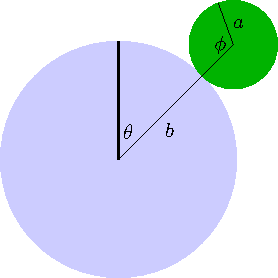
\includegraphics{May2022/1-2.pdf}
\end{center}

}

\sol{

Taking our origin at the center of the larger cylinder, we can write the position vector of the smaller cylinder as
\begin{align}
    \vec{r} = r ( \sin{\theta} \vu*{x} + \cos{\theta} \vu*{y} ) \Rightarrow \dot{\vec{r}} = r \dot{\theta} ( \cos{\theta} \vu*{x} - \sin{\theta} vu*{y} ) \Rightarrow v^2 = r^2 \dot{\theta}^2
,\end{align}
where $r = a + b$.
The kinetic energy
\begin{align}
    T = \frac{m v^2}{2} + \frac{I \omega^2}{2} = \frac{m v^2}{2} + \frac{1}{2} \Big( \frac{1}{2} m a^2 \Big) \Big( \frac{v^2}{a^2} \Big) = \frac{3 m v^2}{4}
.\end{align}
Therefore, the Lagrangian
\begin{align}
    L = \frac{3 m r^2 \dot{\theta}^2}{4} - m g r \cos{\theta}
.\end{align}
From this, we find the equation of motion
\begin{align}
    \eqbox{ \ddot{\theta} - \frac{2 g}{3 r} \sin{\theta} = 0 }
.\end{align}


}


\prob{1.3}{

A particle of mass $M$ is attached by a massless rod of length $a$ to a small ring of mass $m$, free to slide on a fixed horizontal bar.
The string moves in the vertical plane through the bar.

\begin{center}
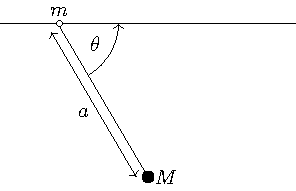
\includegraphics{May2022/1-3.pdf}
\end{center}

\begin{parts}
    \item Write down the Lagrangian and Euler-Lagrange equations for the system.

    \item Find conserved quantities.

    \item Find frequency of small oscillations, if any.
\end{parts}

}

\sol{

(a) Let $x$ denote the position of the mass $m$ and $X,Y$ denote the coordinates of the mass $M$.
We can express
\begin{align}
    X = x + a \cos{\theta}, \quad Y = - a \sin{\theta}
.\end{align}
The Lagrangian
\begin{align}
\eqbox{
\begin{aligned}
    L &= \frac{m \dot{x}^2}{2} + \frac{M}{2} ( \dot{X}^2 + \dot{Y}^2 ) - M g Y \\
      &= \frac{(m + M) \dot{x}^2}{2} + \frac{M}{2} ( a^2 \dot{\theta}^2 - 2 a \dot{x} \dot{\theta} \sin{\theta} ) + M g a \sin{\theta}
\end{aligned}
}
.\end{align}
The equations of motion are given as follows:
\begin{align}
\eqbox{
\begin{aligned} 
    \dv{t} \Big[ (m + M) \dot{x} - M a \dot{\theta} \sin{\theta} \Big] = \dv[2]{t} \Big[ (m+M) x + M a \cos{\theta} \Big] &= 0 \\
    M a^2 \ddot{\theta} - M a ( g + \dot{x} \dot{\theta} ) \cos{\theta} &= M a \ddot{x} \sin{\theta}
.\end{aligned}
}
\end{align}


(b) One can see above that the momentum conjugate to $x$ is conserved:
\begin{align}
    p_x = \dv{L}{\dot{x}} = (m + M) \dot{x} - M a \dot{\theta} \sin{\theta}
.\end{align}
Notice that this is just the $x$ component of the center of mass momentum.
Obviously, we also have energy conservation.


(c) If we insert the conserved momentum into the equation of motion for $\theta$ above, we have
\begin{align}
    M a^2 \Big( 1 - \frac{M}{m + M} \sin^2{\theta} \Big) \ddot{\theta} - \frac{M a p_x}{m + M} \dot{\theta} \cos{\theta} - M a g \cos{\theta} = 0
.\end{align}
If we consider small oscillations such that $\phi = \pi / 2 - \theta \ll 1$, we obtain
\begin{align}
    \ddot{\phi} + \Big( 1 + \frac{M}{m} \Big) \frac{g}{a} \phi = 0
.\end{align}
Notice that we neglected the term $\dot{\theta} \cos{\theta}$ since we have a product of small quantities.
From this, we find the frequency of small oscillations to be
\begin{align}
    \eqbox{ \omega^2 = \sqrt{\Big( 1 + \frac{M}{m} \Big) \frac{g}{a}} }
.\end{align}
Notice that this reduces to the usual pendulum result when $m \gg M$, implying that the suspension point moves very little compared to the hanging mass.

}


\prob{1.4}{

Two bodies move under the influence of the potential $V(r) = k r^{\alpha}$ where $\vb*{r}$ is the relative coordinate and $k$ and $\alpha$ are constants.

\begin{parts}
    \item If $\vb*{r} = \vb*{f}(t)$ is a solution of the equation of motion, show that $\vb*{r} = \lambda \vb*{f}(\lambda^{\sigma} t)$ is also a solution for any $\lambda$ provided $\sigma$ is suitably chosen.

    \item Apply the result of part (a) to the cases $\alpha = 2$ (harmonic oscillator) and $\alpha = -1$ (Kepler problem).
    Comment on the results and on the properties you can derive from them.
\end{parts}

\textbf{Hint}: Use $m \ddot{\vb*{r}} = - \nabla V(\vb*{r})$.

}

\sol{

(a) Let us denote $\vb*{r}' = \lambda \vb*{r}(\tau)$, where $\tau = \lambda^{\sigma} t$.
Observe that
\begin{align}
    \dv{t} = \dv{\tau}{t} \dv{\tau} = \lambda^{\sigma} \dv{\tau} \Rightarrow \dv[2]{t} = \lambda^{2 \sigma} \dv[2]{\tau}
.\end{align}
Additionally,
\begin{align}
    \pdv{r'} = \pdv{r}{r'} \pdv{r} = \frac{1}{\lambda} \pdv{r}
.\end{align}
Thus, for $\vb*{r}'$ to satisfy the desired equation of motion
\begin{align}
    m \dv[2]{t} \vb*{r}' = \lambda^{2 \sigma} \Big( m \dv[2]{\tau} \vb*{r}(\tau) \Big) = - \grad' V(r') = \lambda^{\alpha - 1} \Big( - \grad V(r) \Big)
.\end{align}
In order for $\vb*{r}'(\tau)$ to satisfy the same equation of motion as $\vb*{r}(t)$, we must have
\begin{align}
    \eqbox{ \sigma = \frac{\alpha}{2} - 1 }
.\end{align}


(b) Observe that
\begin{align}
    \eqbox{ \alpha = 2 \Rightarrow \sigma = 0, \quad \alpha = -1 \Rightarrow \sigma = -\frac{3}{2} }
.\end{align}
The latter yields Kepler's third law since $\lambda^{3} = (t / \tau)^2$.

}


\prob{2.1}{

Find the minimal distance between two particles when one of them (having mass $m$) moves from infinity with velocity $v$ and impact parameter $\rho$ towards the second one that is initially at rest (and has mass $M$).
The potential energy of the particle's interaction is given by $U(r) = -U_0 (R/r)^2$, where $r$ is the distance between particles, while $U_0 > 0$ and $R$ are constants.

}

\sol{

At the minimum separation distance, we have
\begin{gather}
    E = \frac{\mu v^2}{2} = \frac{M^2}{2 \mu r^2} - \frac{U_0 R^2}{r^2} = \frac{1}{r^2} \Bigg[ \frac{E m^2 \rho^2}{\mu^2} - U_0 R^2 \Bigg] \nonumber \\
    \eqbox{ r_{\rm min} = \sqrt{\frac{(m + M)^2 \rho^2}{M^2} - \frac{U_0 R^2}{E}} }
.\end{gather}
Notice that if $E$ is small enough, then $r_{min}$ is imaginary, which implies that there is no turning point.
That is, the particles are pulled together with $r = 0$ being unavoidable.

}

\subsection*{Electricity \& Magnetism}
\addcontentsline{toc}{subsection}{Electricity \& Magnetism}

\prob{2.2}{

Consider an infinitely long straight wire along the $z$-axis.
Suppose the wire gets a sudden current by $I(t) = a \delta(t)$, where $a$ is a constant and $\delta(t)$ is the Dirac delta function.
Find

\begin{parts}
    \item the electric and magnetic potentials $\Phi(\vb*{r},t)$, $\vb*{A}(\vb*{r},t)$, and

    \item electric and magnetic fields $\vb*{E}(\vb*{r},t)$, $\vb*{B}(\vb*{r},t)$
\end{parts}

}

\sol{

(a) In the Lorenz gauge, the scalar and vector potentials satisfy wave equations with the charge and current densities as sources, respectively.
That is,
\begin{align}
    \Phi(\vb*{x},t) &= \frac{1}{4 \pi \epsilon_0} \int \dd[3]{\vb*{x}'} \frac{\rho(\vb*{x}', t - |\vb*{x} - \vb*{x}'| / c)}{|\vb*{x} - \vb*{x}'|} \nonumber \\
    \vb*{J}(\vb*{x},t) &= \frac{\mu_0}{4 \pi} \int \dd[3]{\vb*{x}'} \frac{\vb*{J}(\vb*{x}',t - |\vb*{x} - \vb*{x}'| / c)}{|\vb*{x} - \vb*{x}'|}
.\end{align}
The charge density is zero, while the current density reads
\begin{align}
    \vb*{J}(\vb*{x},t) = a \delta(t) \delta(x) \delta(y) \vu*{z}
.\end{align}
Putting these into the potentials, we find
\begin{align}
    \Phi(\vb*{x},t) &= 0 \\
    \vb*{J}(\vb*{x},t) &= \frac{\mu_0}{4 \pi} \vu*{z} \int \dd[3]{\vb*{x}'} \frac{a \delta(t - |\vb*{x} - \vb*{x}'| / c) \delta(x') \delta(y')}{|\vb*{x} - \vb*{x}'|} \nonumber \\
                       &= \frac{\mu_0 a}{4 \pi} \int_{-\infty}^{\infty} \dd{z'} \frac{\delta(t - |\vb*{x} - z' \vu*{z}| / c)}{|\vb*{x} - z' \vu*{z}|}
.\end{align}
Let
\begin{gather}
    f(z') = t - \frac{|\vb*{x} - z' \vu*{z}|}{c} = t - \frac{1}{c} \sqrt{x^2 + y^2 + (z - z')^2} \nonumber \\
f(z') = 0 \Rightarrow z'_{\pm} = z \pm \sqrt{c^2 t^2 - x^2 - y^2} = z \pm \sqrt{c^2 t^2 - s^2} \nonumber \\
\Rightarrow \Big| \pdv{f}{z'}\Big|_{z' = z'_{\pm}} \Big| = \frac{1}{c} \frac{z - z'}{x^2 + y^2 + (z - z')^2} = \pm \frac{\sqrt{c^2 t^2 - s^2}}{c^2 t}
.\end{gather}
Using the property that
\begin{align}
    \int \dd{x} g(x) \delta(f(x)) = \sum_i \frac{g(x_i)}{|f'(x_i)|}
,\end{align}
we find
\begin{align}
\eqbox{
\begin{aligned}
    \Phi(\vb*{x},t) &= 0 \\
    \vb*{A}(\vb*{x},t) &= \frac{\mu_0 a c}{2 \pi \sqrt{c^2 t^2 - s^2}} \vu*{z}
.\end{aligned}
}
\end{align}


(b) The electric and magnetic fields
\begin{align}
\eqbox{
\begin{aligned} 
    \vb*{E} &= - \grad \Phi - \pdv{\vb*{A}}{t} = - \pdv{\vb*{A}}{t} = \frac{\mu_0 a c^2}{2 \pi} \frac{ct}{(c^2 t^2 - s^2)^{3/2}} \vu*{z} \\
    \vb*{B} &= \grad \cross \vb*{A} = - \pdv{A_z}{s} \vu*{\phi} = \frac{\mu_0 a c s}{2 \pi (c^2 t^2 - s^2)^{3/2}} \vu*{\phi}
.\end{aligned}
}
\end{align}


}


\prob{2.3}{

Two thin coaxial rings, each of radius $a$, are a distance $b$ apart, and each uniformly charged with charges $Q_1$ and $Q_2$.
The work required to bring a point charge $q$ from infinity up to the centers of each of the two rings is $W_1$ and $W_2$, respectively.
Show that the charges on the rings are
\begin{align*}
    Q_{1,2} = \frac{4 \pi \epsilon_0 a}{b^2 q} ( a^2 + b^2 )^{1/2} \Big[ (a^2 + b^2)^{1/2} W_{1,2} - a W_{2,1} \Big]
\end{align*}

}

\sol{

The potential on the axis of a ring of radius $a$ with charge $Q$ is given by
\begin{align}
    V(z) = \frac{Q}{4 \pi \epsilon_0} \frac{1}{\sqrt{a^2 + z^2}}
,\end{align}
where $z$ is the distance from the center of the ring.
The work to bring in a test charge $q$ a distance $z$ from the center of the ring is just $W = q V(z)$.
With this, we find that
\begin{align}
    W_1 &= \frac{q}{4 \pi \epsilon_0} \Bigg\{ \frac{Q_1}{a} + \frac{Q_2}{\sqrt{a^2 + b^2}} \Bigg\} \nonumber \\
    W_2 &= \frac{q}{4 \pi \epsilon_0} \Bigg\{ \frac{Q_1}{\sqrt{a^2 + b^2}} + \frac{Q_2}{a} \Bigg\}
.\end{align}
Solving for $Q_1$ in terms of $W_1$ and $Q_2$ we obtain
\begin{align}
    Q_1 = a \Bigg\{ \frac{4 \pi \epsilon_0}{q} W_1 - \frac{Q_2}{\sqrt{a^2 + b^2}} \Bigg\}
.\end{align}
Plugging this into the second expression, we obtain
\begin{gather}
    W_2 = \frac{a}{\sqrt{a^2 + b^2}} W_1 + \frac{q}{4 \pi \epsilon_0} \Big( \frac{1}{a} - \frac{a}{a^2 + b^2} \Big) Q_2 \nonumber \\
    \eqbox{ Q_2 = \frac{4 \pi \epsilon_0 a}{b^2 q} (a^2 + b^2)^{1/2} \Big[ (a^2 + b^2)^{1/2} W_2 - a W_1 \Big] }
.\end{gather}
For $Q_1$, we can interchange the labels $1 \leftrightarrow 2$ to obtain the desired expression.

}


\prob{2.4}{

The region bounded by two concentric spherical surfaces is filled with a uniform charge density $\rho_0$ (constant).
On the inner boundary ($r = a$) of this region, the potential is
\begin{align*}
    \Phi(a,\theta) = V_0 \cos{\theta}
.\end{align*}
On the outer boundary ($r = b$) of this region, the potential is
\begin{align*}
    \Phi(b,\theta) = 2 V_0
.\end{align*}
Find the solution of Poisson's equation in the region $a \leq r \leq b$.

}

\sol{

We can construct the general solution in two pieces.
First, we solve Laplace's equation with the prescribed boundary conditions, which yields $\Phi_1$.
Next, we will solve Poisson's equation with the prescribed charge density and grounded spheres, yielding $\Phi_2$.
The full solution will then just be $\Phi = \Phi_1 + \Phi_2$.

Proceeding with the first part, we write
\begin{align}
    \Phi(\vb*{r}) = \sum_l P_l(\cos{\theta})
    \begin{cases}
        A_l r^l & r < a \\
        B_l r^l + C_l/r^{l+1} & a < r < b \\
        D_l / r^{l+1} & r > b
    .\end{cases}
\end{align}
The boundary conditions are as follows:
\begin{align}
    \Phi(a) = V_0 \cos{\theta}, \quad \Phi(a^{-}) = \Phi(a^{+}), \quad \Phi(b) = 2 V_0, \quad \Phi(b^{-}) = \Phi(b^{+})
.\end{align}
Enforcing them, we find
\begin{align}
\begin{aligned} 
    A_l &= \frac{V_0}{a} \delta_{l 1}, \quad D_l = 2 V_0 b \delta_{l 0} \\
    B_l &= \frac{A_l a^{2l + 1} - D_l}{b^{2l+1} - a^{2l+1}} = \frac{V_0 a^2}{b^3 - a^3} \delta_{l 1} - \frac{2 V_0 b}{b - a} \delta_{l 0} \\
    C_l &= \frac{a^{2l+1} b^{2l+1}}{b^{2l+1} - a^{2l+1}} A_l + \frac{D_l a^{2l+1}}{b^{2l+1} - a^{2l+1}} = \frac{V_0 a^2 b^3}{b^3 - a^3} \delta_{l 1} + \frac{2 V_0 a b}{b - a} \delta_{l 0}
.\end{aligned}
\end{align}
From this, we find
\begin{align}
    \eqbox{ \Phi_1 = V_0 \Bigg\{ \frac{2b}{b - a} \Big( \frac{a}{r} - 1 \Big) + \frac{a^2}{b^3 - a^3} \Big( r + \frac{b^3}{r^2} \Big) \cos{\theta} \Bigg\} }
.\end{align}


Now, we proceed to solve Poisson's equation via Gauss' law:
\begin{align}
    \oint \vb*{E} \cdot \dd{\vb*{a}} = E(r) (4 \pi r^2) = \frac{Q_a + \rho_0(4 \pi r^3 / 3)}{\epsilon_0} \Rightarrow E(r) = \frac{1}{4 \pi \epsilon_0} \frac{Q_a}{r^2} + \frac{\rho_0}{3 \pi \epsilon_0} r
.\end{align}
The potential 
\begin{align}
    \Phi_2 = \int_{r}^{b} E(r') \dd{r'} = \frac{Q_a}{4 \pi \epsilon_0} \Big( \frac{1}{r} - \frac{1}{b} \Big) + \frac{\rho_0}{6 \pi \epsilon_0} (b^2 - r^2)
.\end{align}
Imposing that the inner sphere is also grounded, we find
\begin{align}
    Q_{a} = -\frac{4}{3} \rho_0 a b (a + b)
,\end{align}
and
\begin{align}
    \eqbox{ \Phi_2 = -\frac{\rho_0}{3 \pi \epsilon_0} \Bigg\{ a b (a + b) \Big( \frac{1}{r} - \frac{1}{b} \Big) - \frac{1}{2} ( b^2 - r^2 ) \Bigg\} }
.\end{align}

}


\prob{3.1}{

The $\phi$ particle, which is a bound state $\bar{s}s$ of strange quarks, has mass approximately equal to $1.02~{\rm GeV}/c^2$.

\begin{parts}
    \item What is the minimal (``threshold'') energy of electrons necessary to produce $\phi$ particles in the reaction $ep \rightarrow ep\phi$ at JLab electron accelerator?

    \item What is the velocity and energy (in laboratory frame) of $\phi$ particles produced at threshold?
\end{parts}

}

\sol{

(a) The threshold energy is defined such that
\begin{gather}
    \sqrt{s} = \sqrt{m_{e}^2 + m_p^2 + 2 m_p ( m_e + T ) } = m_e + m_p + m_\phi \nonumber \\
    \Rightarrow \eqbox{ T = \frac{(m_e + m_p + m_\phi)^2 - ( m_e^2 + m_p^2 )}{2 m_p} - m_e = m_{\phi} \Big( 1 + \frac{m_\phi + 2 m_e}{2 m_p} \Big) \approx 1.5~{\rm GeV} }
.\end{gather}

(b) The velocity and energy of the $\phi$ particles produced at threshold in the lab frame are determined by the Lorentz factor, which can be determined by conservation of energy in the lab frame:
\begin{gather}
    m_e + T + m_p = \gamma ( m_e + m_\phi + m_p ) \nonumber \\
    \Rightarrow \gamma = \frac{m_e + m_p + T}{m_e + m_\phi + m_p} = 1 + \frac{m_\phi(m_\phi + 2 m_e)}{2 m_p ( m_e + m_p + m_\phi )} \approx \frac{5}{4}
.\end{gather}
From this, we find the energy of the $\phi$ particle in the lab frame to be
\begin{align}
    \eqbox{ E_\phi = \gamma m_\phi \approx \frac{5}{4} m_\phi }
.\end{align}
The velocity of the $\phi$ particle in the lab frame is given by
\begin{align}
    \eqbox{ \beta = \sqrt{1 - \frac{1}{\gamma^2}} \approx \sqrt{1 - \frac{16}{25}} = \frac{3}{5} }
.\end{align}

}


\prob{3.2}{

An infinitely long, nonconducting solid cylinder of radius $R$ has a \textbf{nonuniform volume charge density} $\rho(r)$ that is a function of the radial distance $r$ from the axis.
See the diagram below.
Say that this charge density is $\rho(r) = B r^2$, where $B$ is a constant with units of $\mu{\rm C}/m^5$.
Use Gauss' law to find the magnitude $E$ of the resulting electric field when

\begin{parts}
    \item $0 < r < R$, and

    \item $r > R$.
\end{parts}

Express your answers in terms of $B$, $r$, $R$, and any constants.

\begin{center}
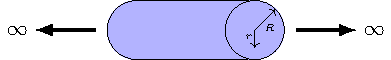
\includegraphics{May2022/3-2.pdf}
\end{center}

}

\sol{

We can determine the electric field using Gauss' law and a cylindrical surface as follows:
\begin{gather}
    \oint \vb*{E} \cdot \dd{\vb*{a}} = E(r) (2 \pi r l) = \frac{1}{\epsilon_0} \int \dd[3]{\vb*{r}} \rho(\vb*{r}) = \frac{2 \pi l}{\epsilon_0} \int_{0}^{r} r' \rho(r') \dd{r'} = \frac{2 \pi l B}{\epsilon_0} \int_{0}^{r} r'^3 \Theta(r' < R) \nonumber \\
    \eqbox{ \vb*{E} = \frac{B}{4 \epsilon_0} \frac{{\rm min}^{4}(r,R)}{r} }
.\end{gather}

}


\prob{3.3}{

A plane electromagnetic wave with frequency $\omega$ traveling in vacuum along the $z$-axis (from $-\infty$) is given by
\begin{align*}
    \vb*{E}_{\rm in}(\vb*{r},t) &= E_{0 ,\rm in} \vu*{x} \exp[i(kz - \omega t)] \\
    \vb*{B}_{\rm in}(\vb*{r},t) &= E_{0,\rm in} \vu*{y} \exp[i(kz - \omega t)]
,\end{align*}
where $k = \omega/c$ and $c$ is the speed of light (Gaussian units).
At $z = 0$, the wave encounters an interface with a semi-infinite, linear dielectric medium filling the entire half-space $z > 0$.
This medium has a dielectric constant (relative electric permittivity) $\epsilon > 1$ but unit magnetic permeability $\mu = 1$ and hence $\vb*{B} = \vb*{H}$.
As a consequence, the medium has an index of refraction $n = \sqrt{\epsilon} > 1$ and a propagation speed $c / n < c$.
Therefore, the transmitted part of the electromagnetic wave in the medium has an electric field given by
\begin{align*}
    \vb*{E}_{\rm tr}(\vb*{r},t) &= E_{0 ,\rm tr} \vu*{x} \exp[i(nkz - \omega t)]
.\end{align*}
Finally, because of the boundary conditions (see below), there must also be a reflected wave going in the negative $z$-direction, with electric field
\begin{align*}
    \vb*{E}_{\rm re}(\vb*{r},t) &= E_{0 ,\rm re} \vu*{x} \exp[-i(kz + \omega t)] \\
\end{align*}

\begin{parts}
    \item Determine the amplitudes $B_{0,\rm tr}$ and $B_{0,\rm re}$ of the magnetic fields of the transmitted and reflected waves,
    \begin{align*}
        \vb*{B}_{\rm tr}(\vb*{r},t) &= B_{tr} \vu*{y} \exp[i(nkz - \omega t)] \\
        \vb*{B}_{\rm re}(\vb*{r},t) &= B_{0 ,\rm re} \vu*{y} \exp[-i(kz + \omega t)] \\
    \end{align*}
    in terms of the corresponding amplitudes $E_{0,\rm tr}$ and $E_{0,\rm re}$. (It is best to use the last of Maxwell's equations, $\nabla \times \vb*{E} + \frac{1}{c} \frac{\partial \vb*{B}}{\partial t} = 0$.)

    \item Using the requirement that \textbf{both} the sum of all electric fields and the sum of all magnetic fields must be continuous at $z = 0$ (why?), determine the relative size of the amplitudes $E_{0,\rm tr}$ and $E_{0,\rm re}$ in terms of $E_{0,\rm in}$.

    \item Calculate the amplitude of the Poynting vector, $\vb*{S}_0 = \frac{c}{4\pi} \vb*{E}_0 \times \vb*{B}_0$, for all three waves, and show that energy is conserved (\textit{i.e.} as much energy is carried in by the incoming wave per unit time as the reflected and transmitted waves carry out).
\end{parts}

}

\sol{

(a) Since we assume harmonic time-dependence, we have
\begin{align}
    \vb*{B} = - \frac{i c}{\omega} \grad \cross \vb*{E} = -\frac{i \omega}{\omega} \pdv{E_x}{z} \vu*{y}
.\end{align}
Thus
\begin{align}
    \eqbox{ B_{0,\rm in} = \frac{k c}{\omega} E_{0,\rm in} = E_{0,\rm in}, \quad B_{0,\rm tr} = n E_{0,\rm tr}, \quad B_{0,\rm re} = - E_{0,\rm re} }
.\end{align}


(b) The boundary conditions at the interface are as follows:
\begin{gather}
    (\vb*{D}_1 - \vb*{D}_2) \cdot \vu*{z} = \vb*{E}_{1,z} - \epsilon \vb*{E}_{2,z} = 0 \\
    ( \vb*{E}_1 - \vb*{E}_2 ) \cross \vu*{z} = - (E_{1,x} - E_{2,x}) \vu*{y} + (E_{1,y} - E_{2,y}) \vu*{x} = 0 \\
    (\vb*{B}_1 - \vb*{B}_2) \cdot \vu*{z} = B_{1,z} - B_{2,z} = 0 \\
    ( \vb*{H}_1 - \vb*{H}_2 ) \cross \vu*{z} = - (B_{1,x} - B_{2,x}) \vu*{y} + (B_{1,y} - B_{2,y}) \vu*{x} = 0
.\end{gather}
The conditions on the components perpendicular to the interface are trivially satisfied, and the rest yield that the parallel components of the field are continuous, which in turn imply that the net fields in each media are the same:
\begin{align}
    E_{0,\rm in} + E_{0,\rm re} = E_{0,\rm tr} \\
    E_{0,\rm in} - E_{0,\rm re} = n E_{0,\rm tr}
.\end{align}
Solving, we find
\begin{align}
    \eqbox{ \frac{E_{0,\rm re}}{E_{0,\rm in}} = \frac{n-1}{2}, \quad \frac{E_{0,\rm tr}}{E_{0,\rm in}} = \frac{n+1}{2} }
.\end{align}


(c) The Poynting vector for each wave
\begin{align}
\begin{aligned} 
    \vb*{S}_{0,\rm in} = \frac{c}{4 \pi} |E_{0,\rm in}|^2 \vu*{z} \\
    \vb*{S}_{0,\rm re} = -\frac{c}{4 \pi} |E_{0,\rm re}|^2 \vu*{z} \\
    \vb*{S}_{0,\rm tr} = \frac{c}{4 \pi}  n^2 |E_{0,\rm tr}|^2 \vu*{z}
\end{aligned}
.\end{align}
The sum of the amplitudes of these vectors (dropping the factors of $c/4\pi$ for brevity) is 
\begin{align}
    \eqbox{ |E_{0,\rm in}|^2 + |E_{0,\rm re}|^2 = |E_{0,\rm in}|^2 \Big( 1 + \frac{n - 1}{2} \Big) = |E_{0,\rm in}|^2 \frac{n + 1}{2} = |E_{0,\rm tr}|^2 }
.\end{align}


}

\subsection*{Quantum Mechanics}
\addcontentsline{toc}{subsection}{Quantum Mechanics}

\prob{3.4}{

A particle of mass $m$ is trapped by a very thin spherical shell of radius $R$ modeled by the potential $U(r) = -V \delta(r - R)$ with $V > 0$.
Consider only the s-state with zero orbital momentum and obtain:

\begin{parts}
    \item The equation for the ground state energy of the bound state.

    \item The critical radius $R_c$ below which the bound state in the well disappears.
\end{parts}

}

\sol{

Schr\"{o}dinger's equation in spherical coordinates takes the form
\begin{align}
    -\frac{\hbar^2}{2 m r^2} \pdv{r} r^2 \pdv{\psi}{r} + \Bigg[ \frac{\vb*{L}^2}{2 m r^2} + V(r) \Bigg] \psi = E \psi
.\end{align}
Writing $\psi(\vb*{r}) = R(r) Y_{lm}(\Omega)$, the Schr\"{o}dinger equation reduces to
\begin{align}
    \frac{1}{r^2} \dv{r} r^2 \dv{R}{r} - \Bigg[ \frac{l(l + 1)}{r^2} + v(r) \Bigg] R = -\epsilon R
,\end{align}
where $v(r) = 2 m V(r) / \hbar^2$ and $\epsilon = 2 m E / \hbar^2$.
Let us write $R(r) = u(r) / r$.
The reduced radial equation is then
\begin{align}
    u_{El}''(r) + \Bigg[ \epsilon - \frac{l(l+1)}{r^2} - v(r) \Bigg] u_{El}(r) = 0
.\end{align}
The s-wave equation in the $\delta$-function potential reads
\begin{align}
    u_{E0}''(r) + \Big[ \epsilon + v \delta(r - R) \Big] u_{E 0}(r) = 0
.\end{align}
Separating into two regions, we have
\begin{align}
    u(r) = \begin{cases}
        A \cosh(\kappa x) + B \sinh(\kappa x) & x < R \\
        C e^{-\kappa x} & x > R
    ,\end{cases}
\end{align}
where $\kappa = \sqrt{|\epsilon|}$.
Since we consider a bound state $\epsilon < 0$.
We have three boundary conditions:
\begin{align}
    &(1): ~ u(r \rightarrow 0) \rightarrow 0 \Rightarrow A = 0 \\
    &(2): ~ u(R^{-}) = u(R^{+}) \Rightarrow B \sinh(\kappa R) = C e^{-\kappa R} \\
    &(3): ~ u'(R^{+}) - u'(R^{-}) = -v u(R) \Rightarrow -\kappa \Big[ C e^{-\kappa R} + B \cosh(\kappa R) \Big] = -v C e^{-\kappa R}
.\end{align}
The first condition is because our system behaves as if the potential is infinite in the region $r < 0$.
From these equations, the condition on the energy of the bound state takes the form of the following transcendental equation:
\begin{align}
    \eqbox{ \frac{\sinh(\kappa R)}{\sinh(\kappa R) + \cosh(\kappa R)} = \frac{1}{2} \Big( 1 - e^{-2 \kappa R} \Big) = \frac{\kappa}{v} }
.\end{align}


(b) There is always a solution at $\kappa = 0$, which implies $E = 0$ but violates our original assumptions which we used to construct our wave function.
Thus, we discard it and look for solutions with $\kappa > 0$.
Notice, however, that the left-hand-side is a constant minus a decreasing exponential, while the right-hand side is a linear function with positive slope.
Both are monotonically increasing functions, but the left-hand-side has a monotonically decreasing derivative while the right-hand-side has a constant slope of $1/v$.
Thus, there will not be a second solution if
\begin{align}
    \eqbox{ \dv{\kappa} \frac{1}{2} \Big( 1 - e^{-2 \kappa R} \Big) \Big|_{\kappa = 0} = R < \frac{1}{v} = R_c }
.\end{align}

}

\prob{4.1}{

An electron is at a fixed position in an oscillating magnetic field
\begin{align*}
    \vb*{B}(t) = B_0 \cos(\omega t) \vu*{z}
,\end{align*}
wherer $B_0$ and $\omega$ are constants.

\begin{parts}
    \item Write down the Hamiltonian for this system.

    \item The electron is at time $t = 0$ in the spin state with eigenvalue $\hbar/2$ with respect to the $x$-axis.
    Determine the spin state of the electron at later times.

    \item Obtain the probability of obtaining $-\hbar/2$ if one measures $S_x$.
\end{parts}

}

\sol{

(a) The Hamiltonian for this system is
\begin{align}
    \eqbox{ H = - \vb*{\mu} \cdot \vb*{B} = - \frac{g_e e}{2 m c} B_0 \cos(\omega t) S_z }
.\end{align}

(b) Since the Hamiltonian commutes with itself at different times, the time evolution operator
\begin{align}
    U(t) = e^{-\frac{i}{\hbar} \int_{0}^{t} H(t) \dd{t}} = e^{i \lambda(t) \sigma_z}
,\end{align}
where $\lambda(t) = (\omega_0 / \omega) \sin(\omega t)$ and $\omega_0 = g_e e B_0 / (4 m c)$.
The state at an arbitrary time $t$ is then
\begin{align}
    \eqbox{ \ket{\psi(t)} = e^{i \lambda(t) \sigma_{z}} \ket{+} = e^{i \lambda(t)} \ket{+} }
.\end{align}

(c) From the above work, we can see that the probability of obtaining $-\hbar / 2$ upon measurement of $S_x$ is just
\begin{align}
    \eqbox{ P(S_x = \hbar/2) = |\ip{+_x}{+}|^2 = \Big| \frac{1}{\sqrt{2}} e^{i \lambda(t)} \Big|^2 = \frac{1}{2} }
.\end{align}

}


\prob{4.2}{

Define a coherent state
\begin{align*}
    \ket{\alpha} = \exp( -\frac{|\alpha|^2}{2} ) \sum_{n=0}^{\infty} \frac{\alpha^n}{\sqrt{n!}} \ket{n}
,\end{align*}
where $\alpha$ is an arbitrary complex number and $\ket{n}$ is the eigenstate of the harmonic oscillator of energy $\hbar \omega (n + 1/2)$.

\begin{parts}
    \item Show that $\bra{\alpha}\ket{\alpha} = 1$ and $\ket{\alpha} = \exp(-|\alpha|^2/2) \exp(\alpha a^{\dagger}) \ket{0}$.

    \item Show that coherent states are eigenstates of the annihilation operator $a \ket{\alpha} = \alpha \ket{\alpha}$.
\end{parts}

}

\sol{

(a) We can prove that the coherent state is normalized as follows:
\begin{align}
    \eqbox{ \ip{\alpha}{\alpha} = e^{-|\alpha|^2} \sum_{n=0}^{\infty} \sum_{m=0}^{\infty} \frac{\alpha^{* \, n} \alpha^{m}}{\sqrt{n! \, m!}} \ip{n}{m} = e^{-|\alpha|^2} \sum_{n=0}^{\infty} \frac{(|\alpha|^2)^{n}}{n!} = 1 }
.\end{align}
Next, we prove the form of $\ket{\alpha}$ in terms of the raising operator:
\begin{align}
    \eqbox{ \ket{\alpha} = e^{-|\alpha|^2/2} \sum_{n=0}^{\infty} \alpha^{n} (\alpha a^{\dagger})^{n} \ket{0} = e^{-|\alpha|^2/2} e^{\alpha a^{\dagger}} \ket{0} }
,\end{align}
where we have used that $a^{\dagger} \ket{n} = \sqrt{n+1} \ket{n+1}$ and $\ket{n} = (a^{\dagger})^{n} \ket{0} / \sqrt{n!}$.

(b) Observe that
\begin{align}
\eqbox{
\begin{aligned} 
    a \ket{\alpha} &= e^{-|\alpha|^2/2} \sum_{n=0}^{\infty} \frac{\alpha^{n}}{\sqrt{n!}} a \ket{n} = e^{-|\alpha|^2/2} \sum_{n=1}^{\infty} \frac{\alpha^{n}}{\sqrt{(n-1)!}} \ket{n-1} \nonumber \\
                   &= e^{-|\alpha|^2/2} \sum_{n=0}^{\infty} \frac{\alpha^{n+1}}{\sqrt{n!}} \ket{n} = \alpha \ket{n}
.\end{aligned}
}
\end{align}

}


\prob{4.3}{

Consider a particle of charge $q$ and mass $m$ in one dimension in a harmonic oscillator potential and under the influence of a uniform electric field.
The Hamiltonian reads
\begin{align*}
    \hat{H} = \hat{H}_0 + \hat{V}, \quad \hat{H}_0 = \frac{\hat{p}^2}{2m} + \frac{m \omega^2}{2} \hat{x}^2, \quad \hat{V} = -q E \hat{x}
.\end{align*}
Assume that the electric field is weak, so that a perturbative calculation is permissible.
The eigenenergies and eigenstates of the harmonic oscillator are well known:
\begin{align*}
    \hat{H}_0 \ket{n} = \hbar \omega (n + 1/2) \ket{n} = \epsilon_{n} \ket{n}
.\end{align*}

\begin{parts}
    \item Calculate the correction (up to including second order) to a generic energy level.

    \item Obtain the exact eigenenergies of $\hat{H}$ and compare them with the results obtained in part (a) above.

    \item Without doing any detailed calculation, explain why the third order correction to a generic level vanishes.
\end{parts}

\textbf{Hint}: Note that, if the first-order correction $E_n^{(1)}$ vanishes, then the third-order correction to a non-degenerate energy level due to a perturbation $\hat{V}$ is simply given by
\begin{align*}
    E_n^{(3)} = \sum_{a,b \ne n} \frac{V_{na} V_{ab} V_{bn}}{(\epsilon_a - \epsilon_n)(\epsilon_b - \epsilon_n)}
.\end{align*}

}

\sol{

(a) The first order perturbative correction to the energies
\begin{align}
    E_{n}^{(1)} = -q E \mel{n}{x}{n} = 0
,\end{align}
where we have used that
\begin{align}
    x = \sqrt{\frac{\hbar}{2 m \omega}} ( a^{\dagger} + a ) \Rightarrow \mel{n}{x}{m} = \sqrt{\frac{\hbar}{2 m \omega}} \Big( \sqrt{m + 1} \delta_{n,m+1} + \sqrt{m} \delta_{n,m-1} \Big)
.\end{align}
Next, we consider the second order correction to the energies:
\begin{align}
    E_{n}^{(2)} &= (q E)^2 \sum_{m \ne n} \frac{|\mel{n}{x}{m}|^2}{\epsilon_{n} - \epsilon_{m}} = \frac{(q E)^2}{\hbar \omega} \frac{\hbar}{2 m \omega} \sum_{m \ne n} \frac{|\sqrt{m+1} \delta_{n,m+1} + \sqrt{m} \delta_{n,m-1}|^2}{n - m} \nonumber \\
                &= \frac{(q E)^2}{2 m \omega^2} \Bigg[ n - (n + 1) \Bigg] = \eqbox{ - \frac{(q E)^2}{2 m \omega^2} }
.\end{align}


(b) Observe that
\begin{align}
    H = \frac{p^2}{2m} + \frac{m \omega^2}{2} x^2 - q E x = \frac{p^2}{2m} + \frac{m \omega^2}{2} \Bigg[ x - \Big( \frac{q E}{ m \omega^2} \Big)^2 \Bigg] - \frac{(q E)^2}{2 m \omega^2}
.\end{align}
Thus, the exact energies of this system are
\begin{align}
    \eqbox{ E_n = \hbar \omega ( n + 1/2 ) - \frac{(q E)^2}{2 m \omega^2} }
.\end{align}

(c) We can see that the second order correction calculated in part (a) matches the second term of the exact energies.
Thus, all the higher order corrections must vanish.

}


\prob{4.4}{

Two nonidentical spin-1/2 particles interact via the Hamiltonian
\begin{align*}
    \hat{H} = A( \sigma_z^{(1)} + \sigma_z^{(2)} ) + B \vb*{\sigma}^{(1)} \cdot \vb*{\sigma}^{(2)}
,\end{align*}
where $\sigma_x$, $\sigma_y$, and $\sigma_z$ are the Pauli $\sigma$-matrices and $\vb*{\sigma} = (\sigma_x,\sigma_y,\sigma_z)$.
The ``(1)'' and ``(2)'' superscripts label particles 1 and 2 respectively.
$A$ and $B$ are real constants.

Find the energy eigenvalues.

\textbf{Hint}: Notice that you can classify the states in terms of the eigenstates of the total spin operators $\hat{S}_z = \frac{\hbar}{2}( \sigma_z^{(1)} + \sigma_z^{(2)} )$ and $\hat{S}^2 = \frac{\hbar^2}{4}( \vb*{\sigma}^{(1)} + \vb*{\sigma}^{(2)} )^2$ since they commute with $\hat{H}$.

}

\sol{

We can rewrite the Hamiltonian as
\begin{align}
    H = A \Big( \sigma_z^{(1)} + \sigma_z^{(2)} \Big) + B \Big[ \frac{1}{2} \Big( \sigma_{+}^{(1)} \sigma_{-}^{(2)} + \sigma_{-}^{(1)} \sigma_{+}^{(2)} \Big) + \sigma_{z}^{(1)} \sigma_{z}^{(2)} \Big]
,\end{align}
where $\sigma_{\pm}$ represents the raising and lowering operators.
Observe that the eigenstates are just the tensor product states of the spin states of particles 1 and 2:
\begin{align}
    \eqbox{ H \ket{++} = (2 A + B) \ket{++}, \quad H \ket{\pm \mp} = -B \ket{\pm \mp}, \quad H \ket{--} = (-2A + B) \ket{--} }
.\end{align}
Alternatively, note that the composite angular momentum states are also eigenstates of the Hamiltonian.
The $\ket{1, \pm 1}$ states are already enumerated, so all that remains are the following
\begin{align}
    H \ket{1 0} = -B \ket{1 0}, \quad H \ket{0 0} = -B \ket{0 0}
.\end{align}


}
